\chapter{Overview}
\label{ch_overview}

\section{Software Description}

It is envisaged that the software will be packaged as a source code deliverable with the relevant autotools based scripts to generate a dynamic/shared library and a coresponding static library that implements lattice-based cryptography. The package will also provide a range of additional test applications (in source code) that implement a comprehensive set of unit tests, a set of functional tests and an exhaustive set of known answer tests (KATs).

As the software is delivered as a source code distributable it will be compiled and linked on a target system. In order to achieve an optimised implementation the build system will reconfigure the source code preprocessor definitions as well as the compiler and linker settings in order to best suit the target system.

A number of utilities derived from the functional tests will also be provided that demonstrate the practical use of the library to perform a typical cryptographic task.

\begin{figure}[!h]
\centering
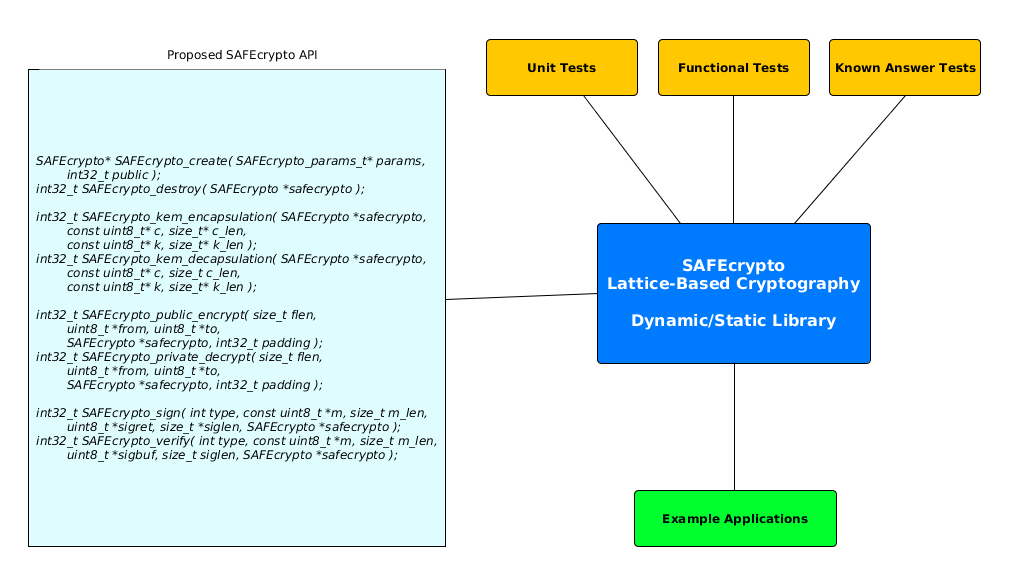
\includegraphics[scale=0.45]{../Resources/SAFEcrypto_structure.png}
\caption{Software structure}
\end{figure}


\section{Project Tools and Build Environment}

\subsection{Programming Language}

The SAFEcrypto software library will be written exclusively in C. In order to provide access to the compiled library in other programming languages a number of bindings will be provided. All C source code produced for the project will be C99 compliant, the ISO/IEC 9899:1999 version of the C programming language.


\subsection{Build Automation}

\textit{A presumption has been made that open-source tools will be preferred as they permit the build system to be deployed at a number of sites in the absence of a cost barrier.}

The build system will be capable of generating a package suitable for use on various platforms and microprocessor architectures with the primary focus being Linux. The generated package will be considered the output of Work Package 6 of the SAFEcrypto project.


\subsection{Code Repository}

The library will be developed at CSIT, as such it will utilise an Innersource GitLab repositiory hosted internally at CSIT as the revision control system for the SAFEcrypto project. In order to provide external access the library will be made publicly available using the SAFEcrypto GitHub repository, where both developers external to CSIT will be able to contribute to the project.


\subsection{Continuous Integration}

\href{https://jenkins.io/}{Jenkins} will be used as the project's CI tool. This will enable both rapid indentification of build errors and provide a consistent and maintainable system on which to create packages. Jenkins will be used to run all automated tests and build functionality, using email reports to notify users of errors.


\subsection{Build System}

The GNU Build System (Autotools) will be used to generate project packages. This build system will require the use of MinGW/MSYS in a Microsoft Windows environment.


\subsection{Compilers}

The GNU Compiler Collection (GCC) will be used on all platforms, using version 5.4 (released June 2016) as a minimum. This will be enforced as a rule within the automated build system to allow developers to standardise the compilation and linking of builds to a minimum standard.


\subsection{Dynamic Analysis Tools}

Dynamic program analysis is the analysis of computer software when running on a microprocessor, offering a user the facility to perform debug memory issues and profile the software. \href{http://valgrind.org/}{Valgrind} will be used to perform memory leak checking, using the test executables to provide sufficient code coverage for the dynamic analysis to be effective.


\subsection{Static Analysis Tools}

Static analysis is a technique that can improve the quality and reliability of software by analysing the source code. \href{http://www.splint.org/}{Splint} will be integrated into the build system for this purpose as an optional build target that developers can use to uncover potential problems.


\subsection{Software Style Formatters}

In order to help maintain a consistent coding style \href{https://www.gnu.org/software/indent/}{GNU Indent} will be used as part of the automated build system to improve the readability of the distributed source code by enforcing a coding style. The committed source code hosted by CSIT GitLab will not utilise automated software style formatting as this will lead to false positive version differences.


\subsection{Documentation Generators}

\href{http://www.doxygen.org/}{Doxygen} will be used for automated code documentation and generation of reference documentation.
